\documentclass[12pt,a4paper]{article}
\usepackage{graphicx}
\usepackage{wrapfig}
\usepackage{textcomp}
\usepackage{multicol}
\usepackage[utf8]{inputenc}

\title{Praktikum Physik - Radioaktivität}
\author{Simon Marti, Patricia Schwab, Mirco Kocher}
\date{18.05.2012}

\begin{document}
\maketitle

\section*{Ziel}
Messung der Abschirmung von radioaktiver Strahlung durch Blei und Aluminium und Berechnung der Massenabsorptionskoeffizienten. Zerfallsreihe von Uran $^{236}U$ mit der Nuklidkarte bestimmen.

\section*{Motivation}
In diesem Experiment wird experimentell nachgewiesen, dass das Absorptionsgesetz seine Berechtigung hat.

\section*{Theorie}
Die Intensit\"at $J$ ist definiert durch Anzahl Zerf\"alle $N$ pro Zeiteinheit $\Delta T$
\begin{equation}
J =\frac{N}{\Delta T}
\end{equation}
Aus dem Absorptionsgesetz mit Absorberdicke $x$ und der Intensit\"at ohne Abschirmung $J_0$
\begin{equation}
J = J_0 e^{-\mu x}
\end{equation}
folgt f\"ur den Massenabsorptionskoeffizienten $\mu_m$
\begin{equation}
\mu_m = - \frac{ln(\frac{J}{J_0})}{x \varrho}
\end{equation}
Die Poisson-Verteilung mit Mittelwert $\lambda$ ist
\begin{equation}
P(k) = \frac{\lambda^k \cdot e^{-\lambda}}{k!}
\end{equation}


\section*{Aufbau und Ablauf}
\begin{center}
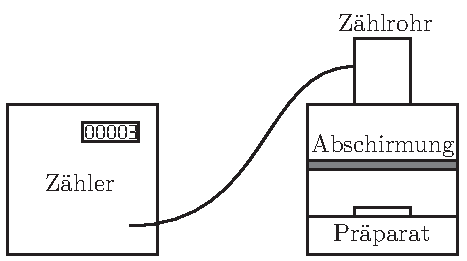
\includegraphics[width=8cm]{illustration.pdf}
\end{center}
Ein radioaktives Präparat wird unter ein Geiger-Müller-Zählrohr gelegt, so dass dazwischen noch dünne Metallplatten zur Abschirmung angebracht werden können. Das Zählrohr ist mit einem elektronischen Zähler verbunden. Für verschiedene Präparate und Abschirmungen wird nun die Impulsrate $A$ gemessen indem Patricia den Zähler eine gewisse Zeit laufen lässt und diese mit einer Stoppuhr misst.


\section*{Aufgabe 1}
\subsection*{Rohdaten}
\[ U_s = 370 \mbox{V} \]

\subsection*{Auswertung}
\begin{center}
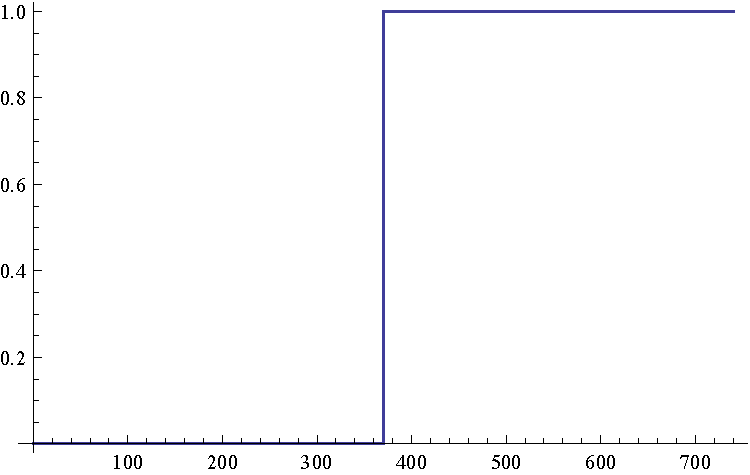
\includegraphics[width=11cm]{diagram1.pdf}
\end{center}


\section*{Aufgabe 2}
\subsection*{Rohdaten}
\[ T = 10 \mbox{s} \]
\begin{tabular}{|r|l|r|l|r|l|r|l|r|l|r|l|}
\hline
$t$&$N$&$t$&$N$&$t$&$N$&$t$&$N$&$t$&$N$&$t$&$N$\\
\hline
10&7&180&89&350&178&520&272&690&352&860&455\\
20&13&190&94&360&186&530&277&700&361&870&458\\
30&16&200&99&370&193&540&279&710&365&880&463\\
40&21&210&105&380&195&550&282&720&371&890&466\\
50&25&220&108&390&198&560&287&730&379&900&472\\
60&29&230&115&400&200&570&291&740&383&910&478\\
70&35&240&118&410&208&580&296&750&389&920&479\\
80&42&250&123&420&210&590&304&760&393&930&480\\
90&47&260&130&430&214&600&308&770&397&940&485\\
100&53&270&130&440&220&610&313&780&403&950&492\\
110&56&280&135&450&225&620&315&790&408&960&497\\
120&59&290&143&460&238&630&322&800&414&970&499\\
130&63&300&149&470&245&640&327&810&418&980&503\\
140&69&310&156&480&250&650&332&820&428&990&507\\
150&72&320&162&490&253&660&335&830&433&1000&509\\
160&79&330&170&500&257&670&342&840&439&1010&512\\
170&87&340&172&510&266&680&349&850&449&1020&520\\
\hline
\end{tabular}

\subsection*{Auswertung}
\[ \overline{N} = 5.079 \mbox{T}^{-1} \]
\[ P(N) = \frac{\overline{N}^N}{e^{\overline{N}}N!} \]
\begin{center}
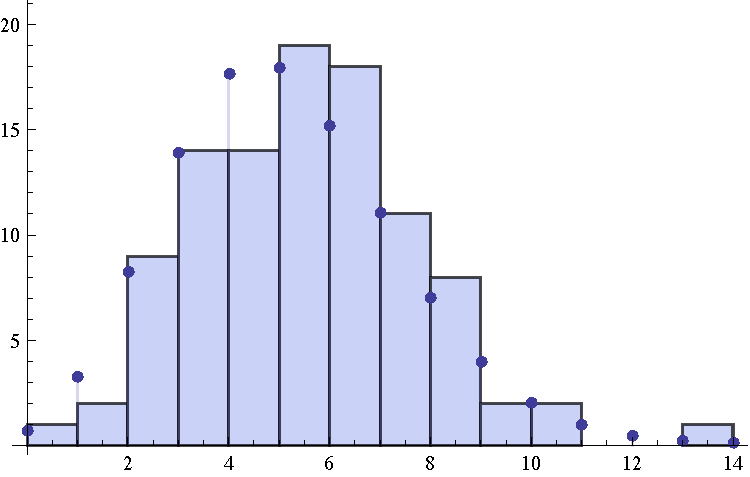
\includegraphics[width=12cm]{diagram2.pdf}
\end{center}

\section*{Aufgabe 3}
$^{238}$U $\rightarrow$  $^{234}$Th $\rightarrow$  $^{234}$Pa $\rightarrow$  $^{234}$U $\rightarrow$  $^{230}$Th $\rightarrow$  $^{226}$Ra $\rightarrow$  $^{222}$Rn $\rightarrow$  $^{218}$Po $\rightarrow$  $^{214}$Pb $\rightarrow$  $^{214}$Bi $\rightarrow$  $^{214}$Po $\rightarrow$  $^{210}$Pb $\rightarrow$  $^{210}$Bi $\rightarrow$  $^{210}$Po $\lor$  $^{206}$Ti $\rightarrow$  $^{206}$Pb  \\
Die Farbe gibt die Zerfallsart an. Dabei ist schwarz stabil, gelb ein $\alpha$-Zerfall, lachs ein $\beta^+$-Zerfall und blau ein $\beta^-$-Zerfall. Ausserdem ist die Halbwertszeit und die freigesetzte Energeie bei dem Zerfall aufgef\"uhrt. Die farbigen Fl\"achen sind ein Mass f\"ur die relative H\"aufigkeit der jeweiligen Zerf\"alle.


\section*{Aufgabe 4}
\subsection*{Rohdaten}
\[ U = 500\mbox{V} \]
\subsubsection*{Nulleffekt}
\begin{tabular}{|r|r|r|}
\hline
$N$&$t$ [s]&J [s$^{-1}$]\\
\hline
4577&16949&0.2700\\
\hline
\end{tabular}

\subsubsection*{${}^{90}$Sr}
\begin{tabular}{|r|l|r|r|r|}
\hline
$x$ [mm]&Material&$N$&$t$ [s]&J [s$^{-1}$]\\
\hline
0&&4978&30.35&163.057\\
2&Aluminium&99&25.86&3.828\\
2&Blei&100&313.73&0.3187\\
\hline
\end{tabular}

\subsubsection*{${}^{60}$Co}
\begin{tabular}{|r|r|r|r|}
\hline
$x$ [mm]&$N$&$t$ [s]&J [s${}^{-1}$]\\
\hline
0&992&138.50&7.162\\
2&1004&155.59&6.453\\
4&1000&183.43&5.222\\
6&1000&191.50&5.221\\
8&1065&223.68&4.761\\
10&1328&306.43&4.334\\
\hline
\end{tabular}


\subsection*{Auswertung}
\subsubsection*{${}^{90}$Sr}
\begin{tabular}{|r|r|r|}
\hline
Material&J$_{Korr}$ [s$^{-1}$]&$\mu /\varrho $ [cm${}^2$g${}^{-1}$]\\
\hline
Aluminium&3.558&7.080\\
Blei&0.0487&3.578\\
\hline
\end{tabular}

\subsubsection*{${}^{60}$Co}
\begin{tabular}{|r|r|r|}
\hline
$x$ [mm]&J$_{Korr}$ [s$^{-1}$]&$\mu /\varrho $ [cm${}^2$g${}^{-1}$]\\
\hline
0&6.892&\\
2&6.18281&0.0479\\
4&5.182&0.0628\\
6&4.952&0.0486\\
8&4.491&0.0472\\
10&4.047&0.0466\\
\hline
\end{tabular}
\begin{center}
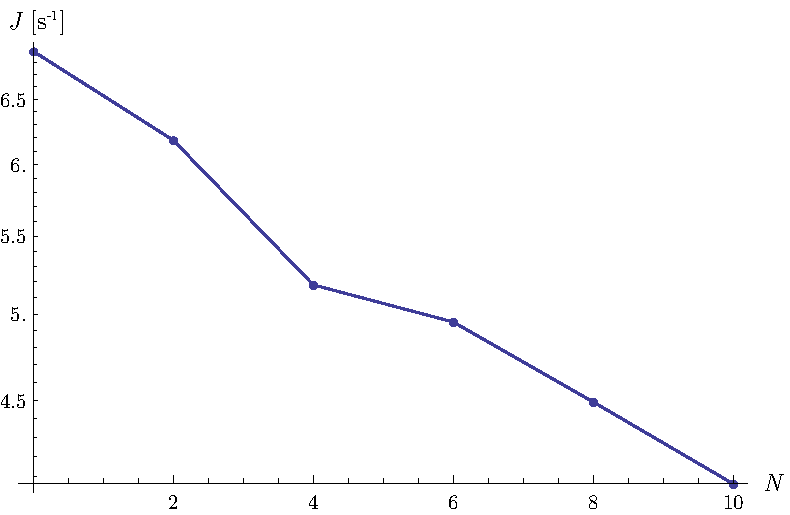
\includegraphics[width=12cm]{diagram4.pdf}
\end{center}

\section*{Diskussion}
Bei der Aufgabe 1 konnten wir die Schwellspannung nur ungenau messen und haben keinen langsamen Anstieg festgestellt, da die Skalierung zu grob war. Ausserdem konnten wir das Ende des Plateaus nicht bestimmen, da unsere maximale Spannung nicht ausgereicht hat.
Die Poisson-Verteilung in Aufgabe 2 stimmt ziemlich gut und man sieht sch\"on, dass es am Anfang stark ansteigt und danach langsamer abflacht.
In Aufgabe 4 ist der Wert von $^{60}Co$ mit 4mm Blei-Abschirmung zu tief. Aus dieser Abweichung folgt auch der ungenaue Massenabsorptionskoeffizienten. Man sieht in der Tabelle zu $^{90}Sr$, dass Blei eine bessere Abschirmung von radioaktiver Strahlung ist.

\end{document}

